\documentclass[dvipdfmx]{jsarticle}
\usepackage{url}
\usepackage{listings}
\usepackage[dvipdfmx]{graphicx}
\usepackage{here}
\usepackage{ascmac}\usepackage{listings, jlisting, color}
\definecolor{OliveGreen}{rgb}{0.0,0.6,0.0}
\definecolor{Orenge}{rgb}{0.89,0.55,0}
\definecolor{SkyBlue}{rgb}{0.28, 0.28, 0.95}
\lstset{
  language={C++}, % 言語の指定
  basicstyle={\ttfamily},
  identifierstyle={\small},
  commentstyle={\smallitshape},
  keywordstyle={\small\bfseries},
  ndkeywordstyle={\small},
  stringstyle={\small\ttfamily},
  frame={tb},
  breaklines=true,
  columns=[l]{fullflexible},
  numbers=left,
  xrightmargin=0zw,
  xleftmargin=3zw,
  numberstyle={\scriptsize},
  stepnumber=1,
  numbersep=1zw,
  lineskip=-0.5ex,
  keywordstyle={\color{SkyBlue}},     %キーワード(int, ifなど)の書体指定
  commentstyle={\color{OliveGreen}},  %注釈の書体
  stringstyle=\color{Orenge}          %文字列
}

\begin{document}
\title{課題3}
\author{ロボ団マスターコース}
\maketitle

\section{はじめに}
\begin{figure}[H]
  \centering
  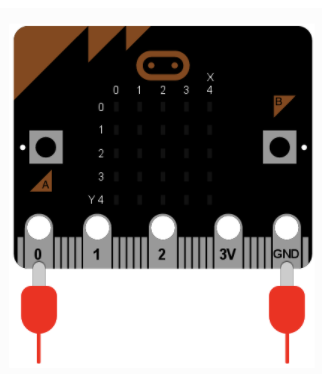
\includegraphics[width=5cm]{1.png}
  \caption{1枚}
\end{figure}

\begin{figure}[H]
  \begin{tabular}{cc}
  \begin{minipage}{.5\textwidth}
      \centering
      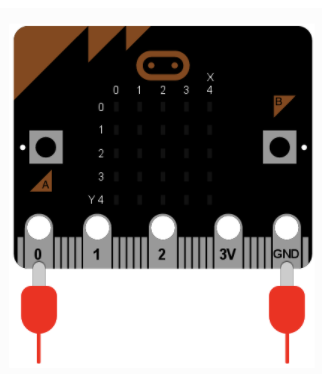
\includegraphics[width=3cm]{1.png}
      \caption{1枚目}
      \label{fig:c}
  \end{minipage}
      \begin{minipage}{.5\textwidth}
      \centering
      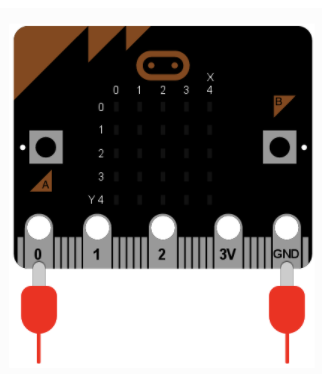
\includegraphics[width=3cm]{1.png}
      \caption{2枚目}
      \label{fig:d}
  \end{minipage}
  \end{tabular}
\end{figure}

\begin{figure}[htpb]
  \begin{tabular}{ccc}
  \begin{minipage}{.33\textwidth}
      \centering
      \includegraphics[width=4cm]{21.pdf}
      \caption{1枚目}
      \label{fig:foo}
  \end{minipage}
      \begin{minipage}{.33\textwidth}
      \centering
      \includegraphics[width=4cm]{21.pdf}
      \caption{2枚目}
      \label{fig:bar}
  \end{minipage}
      \begin{minipage}{.33\textwidth}
      \centering
      \includegraphics[width=4cm]{21.pdf}
      \caption{3枚目}
      \label{fig:hoge}
  \end{minipage}
  \end{tabular}
\end{figure}

\newpage

\section{ソースコード}
\begin{lstlisting} 
printf("階層数を入力:");
scanf("%d", &k);
for(i = 50 - k + 1;i <= 50 + k;i += 2){
    n[i] = 3.;
    n[i+1] = 2.;
}
\end{lstlisting}

\section{箇条書き}
\subsection{パターン1}

\begin{itemize}
\item 音源定位 : 音の発生場所を特定する技術
\begin{itemize}
  \item センサの取り扱い
    \item matlabによるデータ処理
      \item 相互相関関数
        \item 物理学の応用
\end{itemize}
\item 音声認識 : 音声の母音を特定する技術
\begin{itemize}
  \item 周波数解析
    \item 音声情報処理
\end{itemize}
\end{itemize}

\subsection{パターン2}
\begin{enumerate}
\item 時間差\\
自分の右方向から到来した音は、右耳の鼓膜に到着したのち、わずかに遅れて左耳に入る。すなわち同じ音の到着時間に遅延(delay)が発生する。
\item 大きさ\\
同じく右方向から到来した音は右耳では大きく聞こえ、左耳では小さく聞こえる。つまり同じ音が大きく聞こえた方向に音源があるといえる。
\end{enumerate}

\section{数式}
\begin{equation}
R_{ij}(m)=\frac{1}{N-|m|} \sum_{n=0}^{N-1}x_{i}(n)x_{j}(n+m)
\end{equation}

\begin{equation}
\rho_{ij}(m)=\frac{1}{N-|m|} \sum_{n=0}^{N-1}\frac{(x_{i}(n)-\mu_{x_{i}})}{\sigma_{x_i}}\frac{(x_j(n+m)-\mu_{x_j})}{\sigma_{x_j}}
\end{equation}

\section{表}
\begin{tabular}{|c|r|r|r|c|}
\hline
使用音源 & サンプリングレート$[Hz]$ & 量子化ビット数$[bit]$ & データ量$[kB]$ & 実行結果 \\ 
\hline
音源A & $48kHz$ & $16bit$ & $25kB$ & 図1 \\ 
\hline
音源B & $48kHz$ & $16bit$ & $37kB$ & 図2 \\
\hline
音源C & $48kHz$ & $16bit$ & $29kB$ & 図3 \\
\hline
\end{tabular}

\section{囲い}
\begin{itembox}[|]{表名}
  入力ユニット数 + しきい値設定ユニット = 3\\
  中間ユニット数 + しきい値設定ユニット = 3\\
  出力ユニット数 = 1\\
  未知信号の総数 = 4\\
  未知信号 No.1 : 0.000000 0.000000  → 1.000000 1.000000 →0.000000\\
  未知信号 No.2 : 0.000000 1.000000  → 0.000000 0.000000 →1.000000\\
  未知信号 No.3 : 1.000000 0.000000  → 1.000000 1.000000 →1.000000\\
  未知信号 No.4 : 1.000000 1.000000  → 1.000000 0.000000 →0.000000
\end{itembox}

\section{目次みたいの}
\subsection{これ}
\subsubsection{それ}




\end{document}
